\documentclass[conference]{IEEEtran}
\IEEEoverridecommandlockouts

% ==== Fonts & core packages ====
\usepackage{newtxtext,newtxmath} % IEEE推奨Times系
\usepackage{graphicx}
\usepackage{amsmath}
\usepackage{cite}
\usepackage{tikz}
\usetikzlibrary{arrows.meta,positioning,patterns}
\usepackage{xcolor}
\usepackage[hidelinks]{hyperref}

% 図の横幅を安全に抑えるヘルパー
\newcommand{\fitfig}[1]{\resizebox{0.92\linewidth}{!}{#1}}

\title{Educational Perspectives on Complementary FETs (CFET):\\
Evolution Beyond GAA and Open Challenges}

\author{
\IEEEauthorblockN{Shinichi Samizo}
\IEEEauthorblockA{Independent Semiconductor Researcher\\
Project Design Hub, Samizo-AITL\\
\textit{Email:} \href{mailto:shin3t72@gmail.com}{shin3t72@gmail.com}\quad
\textit{GitHub:} \href{https://github.com/Samizo-AITL}{Samizo-AITL}}
}

\begin{document}
\maketitle

\begin{abstract}
This tutorial paper provides an educational overview of emerging
\emph{Complementary FET (CFET)} technology, which vertically stacks nFET and pFET devices beyond Gate-All-Around (GAA) nanosheets.
CFET reframes the CMOS inverter as a \emph{cross-sectional} integration, promising density and delay improvements.
We consolidate structure, electrostatic motivations, layout and delay impacts, fabrication challenges, and modeling limitations, and articulate the pedagogical value of CFET as an open, unresolved technology for semiconductor curricula.
\end{abstract}

\begin{IEEEkeywords}
CFET, GAA, FinFET, nanosheet FET, short-channel effects, scaling, education, tutorial, vertical stacking, PDK.
\end{IEEEkeywords}

% =========================
\section{Introduction}
Scaling has progressed from planar CMOS to FinFET and most recently GAA nanosheet FETs.
Beyond the 2\,nm node, interconnect delay and cell footprint limit further gains despite excellent electrostatics.
CFET stacks nFET and pFET in the vertical dimension so that the cross-section itself constitutes a CMOS inverter, potentially doubling effective standard-cell density while shortening n--p connections.
This paper positions CFET as both a roadmap element and an educational vehicle for device--design co-optimization.

% =========================
\section{Device Evolution: From SCE Relief to Cross-Sectional CMOS}
Scaling history can be viewed as a sequence of innovations in
gate--channel electrostatics. Each generation provided stronger
short-channel control, but also introduced new integration
bottlenecks that motivated the next architectural shift (see Fig.~\ref{fig:evolution}).

\subsection{Planar CMOS: Collapse under SCE}
As gate lengths entered the deep sub-100\,nm regime, planar MOSFETs
suffered severely from short-channel effects (SCE): threshold-voltage
roll-off, drain-induced barrier lowering, large off-state leakage, and
degraded subthreshold slope. Electrostatic control by a single top gate
was insufficient, leading to the collapse of classical planar scaling.

\subsection{FinFET: Three-Sided Gate Recovery}
FinFETs restored scalability by wrapping the gate around
\emph{three} sides of a vertical fin. The enhanced gate coupling
sharpened subthreshold slope, improved variability, and enabled
multi-fin drive current scaling per device. However, the tall/narrow
fin introduced new trade-offs: sensitivity to line-edge roughness,
process variability, and the fact that one side of the channel
remained ungated.

\subsection{GAA Nanosheet: Four-Sided Ideal Control}
Gate-All-Around (GAA) nanosheet FETs extended electrostatics to
\emph{four} sides by surrounding suspended sheets with the gate.
This architecture nearly idealized SCE suppression and variability control,
enabling sub-3\,nm nodes \cite{bsimcmg_sispad2017,loubet_imec_vlsi2019}.
Yet, as device electrostatics became nearly perfect, the performance bottleneck
shifted toward \emph{wiring}: local interconnect resistance/capacitance
(RC) and the lateral footprint of standard cells limited further
delay/energy gains.

\subsection{CFET: Cross-Sectional CMOS Integration}
Complementary FETs (CFETs) address wiring and density limits by stacking
nFET and pFET devices in the \emph{same lateral footprint} and
connecting them vertically. Educational takeaways are:
(i) effective cell density can nearly double by sharing
diffusion/gate footprint across polarities; and
(ii) the critical n-to-p connection in inverters and logic networks is
shortened, reducing local RC and FO1 delay.
In effect, CFET reframes CMOS as a \emph{cross-sectional inverter}
rather than a lateral pair \cite{imec_cfet_iedm2020,colinge_cfet_review2021}.
While promising, CFETs also introduce new integration challenges:
$<5$\,nm alignment tolerance, low thermal budget for sequential processing,
and inter-tier parasitic coupling.

% =========================
\begin{figure}[t]
\centering
\fitfig{%
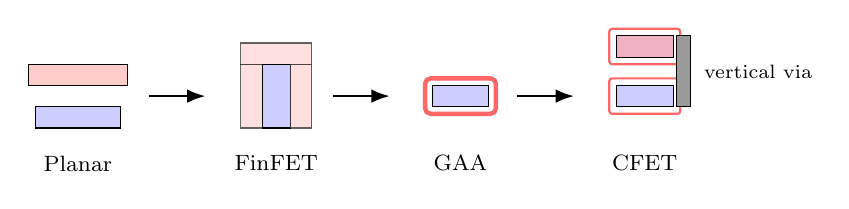
\begin{tikzpicture}[scale=0.9,>=Latex]
% --- Planar ---
\node at (0,-0.8) {\footnotesize Planar};
\draw[fill=blue!20] (-0.6,0) rectangle (0.6,-0.3);
\draw[fill=red!20] (-0.7,0.3) rectangle (0.7,0.6);
\draw (-0.7,0.3) rectangle (0.7,0.6);
% arrow
\draw[->,thick] (1.0,0.15) -- (1.8,0.15);
% --- FinFET ---
\node at (2.8,-0.8) {\footnotesize FinFET};
\draw[fill=blue!20] (2.6,-0.3) rectangle (3.0,0.6);
\draw[fill=red!20,opacity=0.6] (2.3,0.6) rectangle (3.3,0.9);
\draw[fill=red!20,opacity=0.6] (2.3,-0.3) rectangle (2.6,0.6);
\draw[fill=red!20,opacity=0.6] (3.0,-0.3) rectangle (3.3,0.6);
% arrow
\draw[->,thick] (3.6,0.15) -- (4.4,0.15);
% --- GAA ---
\node at (5.4,-0.8) {\footnotesize GAA};
\draw[fill=blue!20] (5.0,0.0) rectangle (5.8,0.3);
\draw[draw=red!60, ultra thick, rounded corners=2pt]
      (4.9,-0.1) rectangle (5.9,0.4);
% arrow
\draw[->,thick] (6.2,0.15) -- (7.0,0.15);
% --- CFET ---
\node at (8.0,-0.8) {\footnotesize CFET};
\draw[fill=blue!20] (7.6,0.0) rectangle (8.4,0.3);
\draw[draw=red!60, thick, rounded corners=1pt] (7.5,-0.1) rectangle (8.5,0.4);
\draw[fill=blue!20!red!30] (7.6,0.7) rectangle (8.4,1.0);
\draw[draw=red!60, thick, rounded corners=1pt] (7.5,0.6) rectangle (8.5,1.1);
\draw[fill=black!40] (8.45,0.0) rectangle (8.65,1.0);
\node[anchor=west,font=\scriptsize] at (8.7,0.5) {vertical via};
\end{tikzpicture}}
\caption{Device evolution: Planar $\to$ FinFET (3-side) $\to$ GAA (4-side) $\to$ CFET (stacked n/p).}
\label{fig:evolution}
\end{figure}

% =========================
\begin{table*}[t]
\centering
\caption{Technology Node Evolution: From GAA to CFET (indicative values, useful for coursework exercises).}
\label{tab:node_scaling}
\begin{tabular}{lcccc}
\hline
\textbf{Node (Year)} & \textbf{Device Architecture} & \textbf{VDD (typ.)} & \textbf{Transistor Density (MTr/mm$^2$)} & \textbf{Notes} \\
\hline
7\,nm (2018)  & FinFET              & 0.70--0.80\,V & 90--100   & Cell height constraints, multi-patterning EUV \\
5\,nm (2020)  & FinFET $\rightarrow$ pre-GAA & 0.65--0.75\,V & 130--170  & First high-volume EUV, RC delay dominant \\
3\,nm (2023)  & GAA nanosheet       & 0.60--0.70\,V & 200--250  & Four-sided electrostatics, variability reduction \\
2\,nm (2025 est.) & GAA production   & 0.55--0.65\,V & 300--400  & Multi-sheet optimization, DTCO critical \\
$<$2\,nm (2027--2030) & CFET (stacked n/p) & 0.50--0.60\,V & 500--700  & Cross-sectional inverter, vertical RC benefit \\
1\,nm-class (2030+) & Sequential/Forksheet CFET & $<$0.50\,V & $>$800 & 3D stacking, thermal-aware BEOL, AI-assisted design \\
\hline
\end{tabular}
\end{table*}

% =========================
\begin{figure*}[!t]
\centering
\fitfig{%
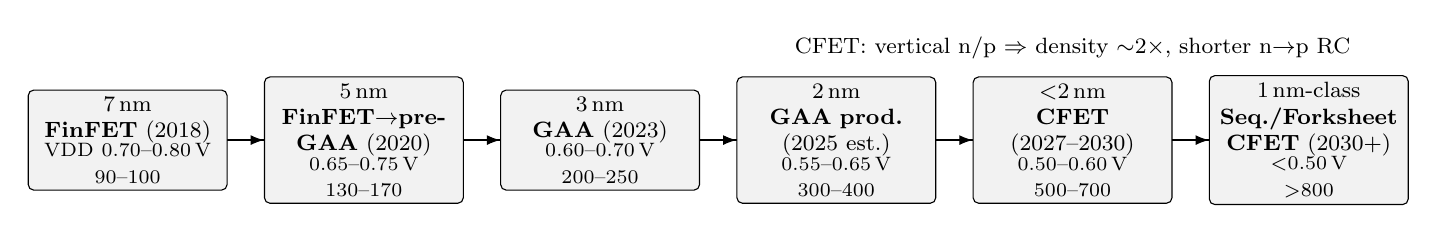
\begin{tikzpicture}[>=Latex, node distance=2.2cm, y=0.65cm]
\tikzset{
  stage/.style={
    draw, rounded corners=2pt, align=center, fill=gray!10,
    minimum width=2.35cm, minimum height=1.05cm,
    inner sep=2.5pt,
    font=\footnotesize, text width=2.35cm
  },
  annot/.style={align=center, font=\scriptsize}
}
\draw[->, semithick] (-0.4,0) -- (16.2,0);
\node[stage] (n7)  at (0,0)   {7\,nm\\ \textbf{FinFET} (2018)\\[-1pt]
  {\scriptsize VDD 0.70--0.80\,V\\ 90--100}};
\node[stage] (n5)  at (3.0,0) {5\,nm\\ \textbf{FinFET$\to$pre-GAA} (2020)\\[-1pt]
  {\scriptsize 0.65--0.75\,V\\ 130--170}};
\node[stage] (n3)  at (6.0,0) {3\,nm\\ \textbf{GAA} (2023)\\[-1pt]
  {\scriptsize 0.60--0.70\,V\\ 200--250}};
\node[stage] (n2)  at (9.0,0) {2\,nm\\ \textbf{GAA prod.} (2025 est.)\\[-1pt]
  {\scriptsize 0.55--0.65\,V\\ 300--400}};
\node[stage] (c20) at (12.0,0){$<$2\,nm\\ \textbf{CFET} (2027--2030)\\[-1pt]
  {\scriptsize 0.50--0.60\,V\\ 500--700}};
\node[stage] (c10) at (15.0,0){1\,nm-class\\ \textbf{Seq./Forksheet CFET} (2030+)\\[-1pt]
  {\scriptsize $<$0.50\,V\\ $>$800}};
\draw[->] (n7) -- (n5);
\draw[->] (n5) -- (n3);
\draw[->] (n3) -- (n2);
\draw[->] (n2) -- (c20);
\draw[->] (c20) -- (c10);
\node[annot] at (12.0,1.8) {\footnotesize CFET: vertical n/p $\Rightarrow$ density $\sim$2$\times$, shorter n$\to$p RC};
\end{tikzpicture}}
\caption{Compact roadmap timeline aligned with Table~\ref{tab:node_scaling}. Values indicative; adapted from IRDS~\cite{irds_2023} and IMEC~\cite{imec_cfet_iedm2020}.}
\label{fig:roadmap_timeline}
\end{figure*}
\vspace{0.6ex}

% =========================
\section{CFET Structural Concepts}
Two integration styles are considered, reflecting a likely roadmap progression:
first the \emph{Sequential CFET} as the initial candidate,
and then the \emph{Forksheet CFET} as a possible successor if inter-tier
interference proves problematic (Figs.~\ref{fig:cfet_stack}, \ref{fig:forksheet}).

\paragraph*{(i) Sequential CFET}
The first integration style expected in practice is the Sequential CFET.
Here, the nFET tier is fabricated first, followed by the pFET tier stacked
above it under a constrained thermal budget. Selective epitaxy/etch and
dielectric isolation are crucial, as is vertical contact to the inverter output.
Because n- and p-devices are stacked in close proximity, however,
concerns arise regarding electrostatic coupling, vertical via parasitics,
and thermal interference between tiers.

\begin{figure}[t]
\centering
\fitfig{%
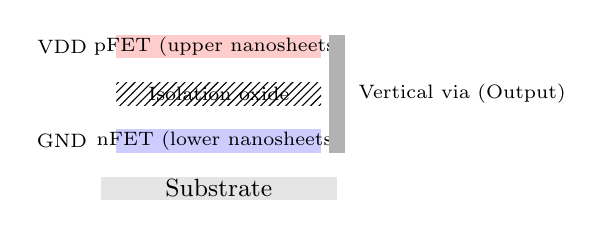
\begin{tikzpicture}[scale=1.0]
% Substrate
\fill[gray!20] (0,0) rectangle (3,0.3);
\node at (1.5,0.15) {\small Substrate};

% nFET
\fill[blue!20] (0.2,0.6) rectangle (2.8,0.9);
\node at (1.5,0.75) {\scriptsize nFET (lower nanosheets)};

% Isolation oxide
\fill[gray!40,pattern=north east lines] (0.2,1.2) rectangle (2.8,1.5);
\node at (1.5,1.35) {\scriptsize Isolation oxide};

% pFET
\fill[red!20] (0.2,1.8) rectangle (2.8,2.1);
\node at (1.5,1.95) {\scriptsize pFET (upper nanosheets)};

% Vertical via
\fill[black!30] (2.9,0.6) rectangle (3.1,2.1);
\node[anchor=west] at (3.15,1.35) {\scriptsize Vertical via (Output)};

% Supply labels
\node[anchor=east] at (-0.05,1.95) {\scriptsize VDD};
\node[anchor=east] at (-0.05,0.75) {\scriptsize GND};
\end{tikzpicture}}
\caption{Sequential CFET cross-section: stacked nFET/pFET with vertical output via.
Current research focuses on managing parasitic coupling and thermal interference in this architecture.}
\label{fig:cfet_stack}
\end{figure}

\paragraph*{(ii) Forksheet CFET}
If interference in Sequential CFETs becomes too severe, a next-step option is the
Forksheet CFET. In this style, n- and p-channels are placed orthogonally and
separated by a dielectric ``fork'' spacer. This geometry helps mitigate
inter-tier parasitics, preserves electrostatic control, and eases routing
congestion.

\begin{figure}[t]
\centering
\fitfig{%
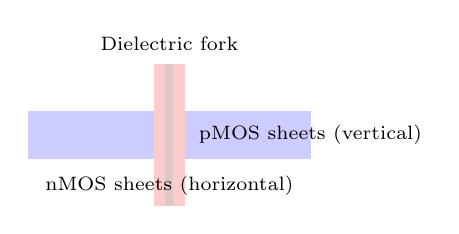
\begin{tikzpicture}[scale=1.0]
% nMOS horizontal region
\fill[blue!20] (0.2,0.0) rectangle (3.8,0.6);
% pMOS vertical region
\fill[red!20] (1.8,-0.6) rectangle (2.2,1.2);
% Dielectric fork (thin)
\fill[gray!45,opacity=0.6] (1.95,-0.6) rectangle (2.05,1.2);

% Labels
\node[anchor=south] at (2.00,1.25) {\scriptsize Dielectric fork};
\node[anchor=west]  at (2.25,0.30) {\scriptsize pMOS sheets (vertical)};
\node[anchor=north] at (2.00,-0.10) {\scriptsize nMOS sheets (horizontal)};
\end{tikzpicture}}
\caption{Forksheet CFET top view: orthogonal n/p nanosheets with a dielectric fork.
This style is envisioned as a follow-up option if Sequential CFET coupling proves too limiting.}
\label{fig:forksheet}
\end{figure}

% =========================
\section{Electrical and Layout Impacts}
CFET integration affects not only cell density but also delay,
variability, and power distribution in ways that extend beyond GAA devices.
Key educational points include:
\begin{itemize}
  \item \textbf{Area efficiency:} By vertically stacking nFET and pFET within the same lateral footprint, inverter density can approach
  nearly $2\times$. This benefit extends to complex logic cells (e.g., NAND/NOR) by co-locating pull-up and pull-down networks in
  the same footprint. Students should recognize how this structural gain cascades into standard-cell library design and physical design
  rules such as \emph{cell height} and \emph{routing pitch}.
  \item \textbf{Delay/energy:} The vertical n-to-p via drastically shortens the inverter’s RC path compared to lateral wiring in GAA.
  Even if individual $I$–$V$ curves remain similar to GAA, FO1 delay and stage energy are improved due to reduced interconnect length.
  This highlights the shift of scaling benefit from device $I$–$V$ to \emph{wiring geometry}.
  \item \textbf{Electrostatics:} Each tier can retain GAA-level control, but inter-tier dielectric/field coupling introduces new parasitics
  (capacitance, via resistance). This provides an excellent tutorial case where device electrostatics interact with circuit parasitics,
  requiring students to think about multi-physics co-optimization.
  \item \textbf{Variability/noise:} Vertical stacking introduces thermal coupling between tiers, causing asymmetric heating of n/p devices.
  Furthermore, VDD and GND partitioning across layers generates uneven IR drop and noise susceptibility. These effects demand new
  placement and routing strategies, illustrating how device innovations ripple up into CAD tool requirements.
\end{itemize}
From a teaching perspective, this section demonstrates how \emph{device-level innovations directly translate into EDA challenges},
making CFET a natural case study in DTCO curricula.

% =========================
\section{Manufacturing Challenges}
Realizing CFETs requires overcoming fabrication hurdles that exceed previous scaling transitions.
Independent n/p work-functions and junctions across stacked tiers demand highly selective epitaxy and etching,
often under low thermal budgets ($<500^{\circ}$C) to avoid damaging the completed tier.
Vertical via alignment must achieve sub-5\,nm overlay, pushing EUV lithography beyond current production standards.
Dielectric isolation must simultaneously suppress dopant diffusion and preserve mechanical integrity across multiple stacked layers.

Recent demonstrations by IMEC indicate that sequential CFETs are feasible at the research level \cite{imec_cfet_iedm2020}.
However, industrial-scale yield, variability control, and long-term reliability remain unresolved.
In particular, \emph{independent threshold-voltage tuning of nFET/pFET tiers} is critical for SRAM stability and large-scale logic integration.
This makes CFET a rich topic for classroom debate on manufacturability versus theoretical scaling.

% =========================
\section{Modeling and EDA Limitations}
Existing compact models such as BSIM-CMG can capture GAA device behavior, but extensions to CFET remain absent.
Key missing aspects include:
\begin{enumerate}
  \item Inter-tier electrostatics and capacitive coupling,
  \item Vertical thermal interactions between stacked devices,
  \item Parasitic RC from vertical vias and tier-to-tier contacts.
\end{enumerate}
Prototype Verilog-A models have been proposed but lack consensus, calibration, and reproducibility.
Furthermore, no open-source CFET-ready PDKs or standard-cell libraries are available, preventing standardized design flows.
From an educational perspective, this modeling gap provides fertile ground for coursework:
students can extend compact models, explore sensitivity analysis, and appreciate the impact of missing parasitics on design predictions.
This gap is also echoed in the IRDS roadmap \cite{irds_2023}.

% =========================
\section{Educational Value}
From a pedagogical perspective, CFET is more than a new device—it is a framework for integrating physics, process, layout, and CAD.
Graduate courses can incorporate:
\begin{itemize}
  \item CFET Verilog-A models as design projects,
  \item Sensitivity studies to inter-tier parasitics,
  \item Placement/routing co-optimization exercises,
  \item Roadmap-based discussions linking IRDS forecasts with design-technology co-optimization (DTCO).
\end{itemize}
Instructors can also differentiate usage scenarios:
undergraduate courses may use CFET as a case study of scaling limits and integration hurdles,
while graduate curricula can involve hands-on modeling, layout co-optimization, and system-level DTCO studies.
This dual-level approach illustrates how CFET can serve as both an introduction to scaling challenges and an advanced platform for design research.

% =========================
\section{Conclusion and Outlook}
CFET reframes CMOS as a stacked, cross-sectional inverter that simultaneously improves density and wiring delay.
Looking forward, several research vectors emerge \cite{colinge_cfet_review2021,irds_2023}:
\begin{itemize}
  \item Forksheet CFET layouts to mitigate inter-tier interference,
  \item 3D sequential stacks under constrained thermal budgets,
  \item Thermal-aware power partitioning across vertical tiers,
  \item Co-optimized BEOL integration to reduce parasitic loading,
  \item AI-driven exploration of design space for DTCO.
\end{itemize}
Embedding CFET into semiconductor curricula not only prepares engineers for the 2030s,
but also fosters critical thinking about unresolved challenges at the scaling frontier---where physics, fabrication, and system design converge.

% ========================
\section*{Acknowledgment}
The author thanks the Project Design Hub community for discussions.

% ========================
\bibliographystyle{IEEEtran}
\bibliography{refs}

% ========================
\section*{Author Biography}
\noindent\textbf{Shinichi Samizo}
received the M.S. degree in Electrical and Electronic Engineering from Shinshu University, Japan.
He worked at Seiko Epson Corporation as an engineer in semiconductor memory and mixed-signal device development, and also contributed to inkjet MEMS actuators and PrecisionCore printhead technology.
He is currently an independent semiconductor researcher focusing on process/device education, memory architecture, and AI system integration.\\[2pt]
\textbf{Contact:} \href{mailto:shin3t72@gmail.com}{shin3t72@gmail.com}, \href{https://github.com/Samizo-AITL}{Samizo-AITL}

\end{document}
